\chapter{評価スコアを推定するモデルの構築}
\thispagestyle{myheadings}

本研究では,UTAU音源ライブラリに対して声質に対する評価スコアを付与するための機械学習モデルを作成する.
それぞれのライブラリの音声から抽出した特徴量と,事前にアンケート調査などによって得られた評価スコアを用い,特徴量から評価スコアを推定するモデルを作成する.
評価スコアの推論には学習データとしてUTAU音源声質アンケートのデータを,モデル作成にはPythonライブラリであるPyCaretを用いた.

\section{特徴量の抽出}
特徴量を抽出するためには,ライブラリを用いて複数の音階で「あ」「い」「う」「え」「お」「ん」と発声した音声ファイルを利用する.
五母音と子音「ん」は連続して発声のできる音素であり,安定して音声の特徴を抽出できる.
音階はA3,D4,G4,C5,F5の5音階を用いる.
複数の音階を用いる特徴量の数を増加させるほか,音声の音域による特徴への影響などを反映できると考えられる.

実際に用いる特徴量としては,MFCC,ZCR,F1〜F4の周波数を採用した.
MFCCは音声の周波数成分を人間の聴覚特性に基づいて変換したものであり,話者認識になどに広く用いられている.
音声の声質に関連すると考えられるため採用し,本研究ではMFCCを64次元まで取得し用いる.
ZCRは音声の振動数を表す指標であり,音の高さやノイズの大きさによって振動数は変化する.
音声の声高を固定した今回の音声であれば,音声の声質に関連する指標として扱えると考え採用した.
音響フォルマントは音声の共振周波数を表す指標であり,母音の識別に用いられる.
同じ音素のフォルマント周波数でも話者の年齢や性別によって変化があり\cite{formant},声の印象に影響があると考えられる.
本研究では各音階と音素ごとのF1〜F4の周波数を取得し用いる.

\section{モデルの構築}
モデルの構築にはPythonライブラリであるPyCaretを用いた.
PyCaretは機械学習モデルの作成を簡略化するためのライブラリであり,データの前処理からモデルの選定,評価までを一連の流れで行える.
UTAU音源声質アンケートの結果はExcelファイルとして提供されている.
このファイルに記載されている240種のUTAU音源ライブラリのうち,現在でもダウンロードが可能であり,必要な音素が収録されていて,かつ利用規約上で研究目的を含む機械学習用途での利用が禁止されていない168ライブラリを対象とした.
各評価スコアを推論の目標として与え,先述の特徴量から評価スコアを推定するモデルを評価スコアの7軸それぞれについて別々に作成した.
学習時には,使用するライブラリから3割をランダムに選びテストデータとして,残りのデータを学習データとして用いた.
学習モデルはPyCaretで選択できる手法のうち,連続モデルの中で学習後のR2値が高かったAdaBoost Regressorを選択した.
これは連続量である特徴量から連続量である評価スコアを推定するため,離散モデルよりも連続モデルの方が適していると考えたほか,離散モデルでの学習を試した際に過学習と見られる状況が多く見られたためである.

\section{UTAU音源ライブラリとUTAU音源声質アンケート}
本研究において探索対象とするUTAU音源ライブラリは,無償で公開されている歌唱用音声合成ソフトであるUTAU上で使用できる音源ファイルであり,ソフトと同じく無償で公開されているものが多い.
UTAUは波形接続と呼ばれる手法を用いており,音声データを切り貼りして音声を合成する.
そのため,UTAU音源ライブラリは主に合成に用いるためにできる限り一定の音程と音量になるように収録された収録者の肉声が収録されている.
収録形式には複数の手法があり,単独音であれば各wavファイルにひらがな1文字に対応する音素が収録されており,連続音(VCV)であれば「あんああいあうあ」\cite{tatsu3shiki}といった形で複数の音素が連続して収録されている.

本研究で実際に特徴量を抽出する際,音声合成は行わずこのwavファイルを直接操作し音声合成の手間を削減した.
必要な音素が収録された音声ファイルのうち,UTAUにおいては子音部とブランクとして指定されるタイミング間の音声を利用した.
この範囲はUTAU上で音声が合成される際母音を伸ばすために用いる範囲であり,一般に安定して同じ声が収録されているため音声の特徴を抽出する上で適していると考えられる.
複数音階の音声の生成には,音階ごとにライブラリで指定されるwavファイルからピッチシフトを行い,音声を生成した.

UTAU音源声質アンケートはニコニコ大百科上で提言されたUTAU音源ライブラリに対する声の特徴を評価するためのアンケート規格であり,現在までにこの規格を用いて250種以上のUTAU音源ライブラリに対してアンケートが行われている.
このアンケートは表\ref{tab:survey}に示す7項目について,それぞれ1から7までの7段階評価で10件以上のアンケート調査を行い,その平均を評価値としている.
アンケートは各UTAU音源ライブラリごとに行われ,表情音源が複数存在する場合は各表情音源ごとに独立してアンケートが行われている.

\begin{table}[htb]
  \centering
  \caption{UTAU音源声質アンケートの評価軸}
  \label{tab:survey}
  \begin{tabular}{c|cc}
    \hline
    評価軸 & 低い値の示す表現語 & 高い値の示す表現語 \\
    \hline
    声の性別 & 女性的 & 男性的 \\
    滑舌 & 舌足らず & はきはき \\
    特有性 & 素直 & 癖がある \\
    声の年齢 & 幼い & 大人びた \\
    透明感 & ノイジー & クリア \\
    声の強さ & 優しい & 力強い \\
    声の明度 & 暗い & 明るい \\
    \hline
  \end{tabular}
\end{table}

UTAU音源ライブラリは数が多い点だけでなく,声質の依存先が生の音声ファイルである点や,音素情報を関連づけるiniファイルが一般的に用いられる形式であるため非常に扱いやすい点,UTAU音源声質アンケートが存在する点が評価できる.
無償で利用できるものがほとんどである点も,多くの合成音声の中から用いたい声を探したい利用者のニーズに合っている.
ライブラリの声質を評価する上で,また利用者からの目線においても都合が良いと考え,本研究の対象として選定した.

\section{結果の評価} \label{sec:eval}
構築したモデルによる推論の精度を評価するため,テストデータに対して推論を行い得た値と実際のアンケートによって得られた値を比較した.
テストデータは先述の通り学習データからランダムに選ばれたデータであり,対象とした168ライブラリの3割にあたる51ライブラリを用いた.
7つの評価軸それぞれについて,テストデータでの精度を評価した結果を図\ref{tab:score_box},図\ref{tab:score_coor}に示す.

\begin{figure}[h]
  \centering
  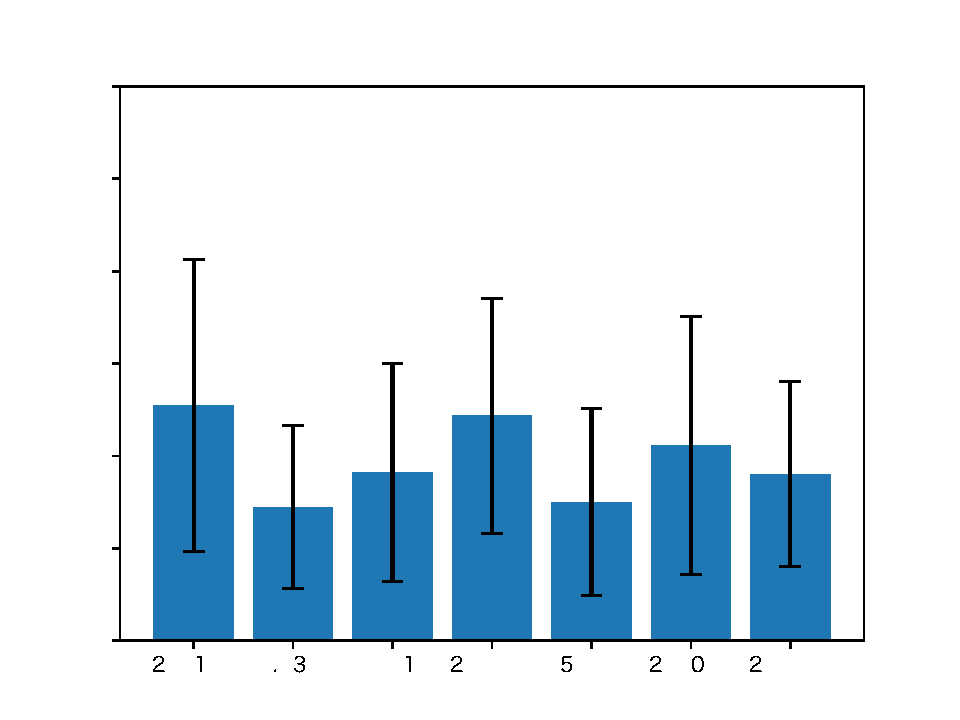
\includegraphics[width=\linewidth]{fig/model_quality_rms.pdf}
  \caption{テストデータとの誤差の二乗平均平方根}
  \label{tab:score_box}
\end{figure}

\begin{figure}[h]
  \centering
  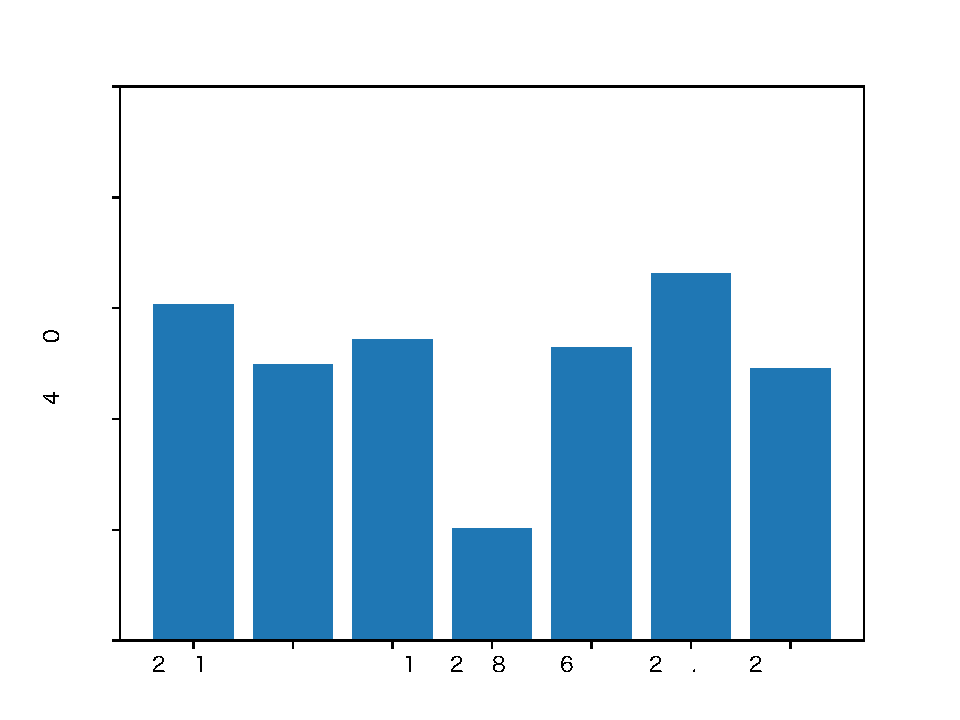
\includegraphics[width=\linewidth]{fig/model_quality_coor.pdf}
  \caption{テストデータとの相関係数}
  \label{tab:score_coor}
\end{figure}

図\ref{tab:score_box}では,横軸は評価軸を,縦軸はテストデータにおける実際の値と推測された値との誤差の二乗平均平方根(RMS),エラーバーは誤差の標準偏差を示している.
RMSは実際の値と推測された値の誤差を示す指標であり,誤差が小さいほど推論の精度が高いと言える.
結果として誤差のRMSは最も高い声の性別で1.3となった.
これは先行研究\cite{dnn}の精度に近く,先行研究にて示された音響特徴量を用いたモデルの精度が再現できたと言える.

図\ref{tab:score_coor}では,横軸は評価軸を,縦軸はテストデータにおける実際の値と推測された値との相関係数を示している.
相関係数は一般に0.7以上であればデータ間に強い相関が,0.4以上であればある程度の相関があるとされ,実際の値と推測された値における相関が強いほど推論の精度が高いと言える.
結果を見ると,最も低い声の年齢は0.20とかなり低いものの,他の評価軸では0.49から0.66程度,最も高い声の強さでは0.66と,ある程度の相関が見られた.

相関係数の最も高い声の強さと最も低い声の年齢において,実際の値と推測された値の散布図を図\ref{fig:scatter}に示す.
図を見ると,声の強さは右肩上がりの傾向が見られ,相関の存在が分かる一方で,声の年齢は点が縦に長く分布しているのが分かる.
これは相関がないことに加え,実際の値はスコア範囲中に広く分布しているにも関わらず,予測された値がおおよそ3〜5と範囲の中央に偏っていることを表している.
この傾向は程度の差はあれど声の性別と声の強さを除く全ての評価軸においても見られ,精度を下げている一因となっている.

\begin{figure}[h]
  \centering
  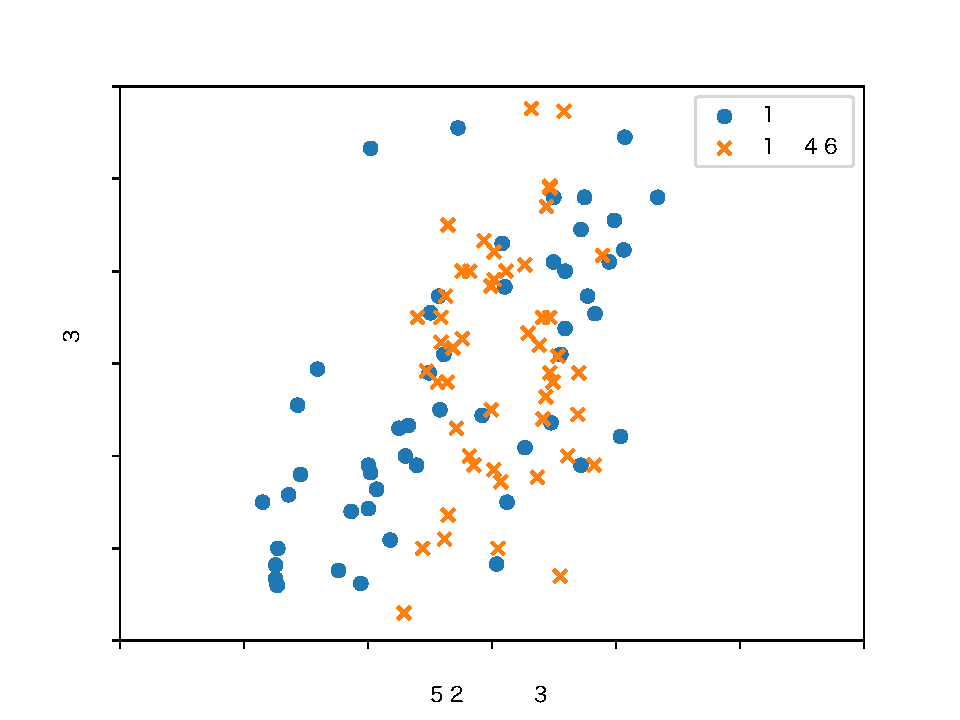
\includegraphics[width=\linewidth]{fig/scatter.pdf}
  \caption{実際の値と推測された値の散布図}
  \label{fig:scatter}
\end{figure}

予測値が中央に偏る現象について,一般にはデータの偏りやモデルの過学習,特徴量の不足などが要因とされている.
学習データを確認したが,テストデータのスコア分布からも分かるように,実際のスコアは広く分布しておりスコア的な偏りは認められなかったほか,モデルの過学習についてもそのような傾向は見られなかった.
一方で,今回用いた音声特徴量が声質の印象に対し十分でなかった可能性がある.
主に母音の音素に対して音階ごとに別々の特徴量を抽出したが,音素間の遷移の特徴などより複雑な特徴量も声の印象に影響していると考えられる.
そのほか先行研究\cite{dnn}では機械学習の手法としてディープラーニングのモデルが採用されていたように,学習手法は複数のものが考えられる.
様々な手法を試し,より適したものに変えることで性能向上の余地があると考えられる.

% Local Variables:
% mode: japanese-LaTeX
% TeX-master: "root"
% End:
